\pdfobjcompresslevel=0\relax
\pdfminorversion=5\relax
\documentclass[a4paper,11pt]{article}

% ---------------------------------------------------------------------
% Language, fonts and page layout
% ---------------------------------------------------------------------
\usepackage[utf8]{inputenc}
\usepackage[T5]{fontenc}
\usepackage{lmodern}
\usepackage[english]{babel}
\usepackage{microtype}

\usepackage[a4paper,left=19mm,right=19mm,top=20.5mm,bottom=20.5mm]{geometry}
\usepackage{indentfirst}

% ---------------------------------------------------------------------
% Tables, figures, colour
% ---------------------------------------------------------------------
\usepackage{float}
\usepackage{array}
\usepackage{tabularx}
\usepackage{booktabs}
\usepackage{multirow}
\usepackage{makecell}
\usepackage{graphicx}
\usepackage{adjustbox}
\usepackage{caption}
\usepackage{subcaption}
\usepackage{amsmath}
\usepackage{xcolor}
\usepackage{tikz}
\usetikzlibrary{arrows.meta,calc,positioning}
\usepackage{pgfplots}
\usepgfplotslibrary{groupplots}
\pgfplotsset{compat=1.17}
\usepackage{enumitem}
\setlist{nosep,leftmargin=1.4em,itemsep=1pt,topsep=2pt}

\newcolumntype{L}[1]{>{\raggedright\arraybackslash}p{#1}}
\newcolumntype{Y}{>{\raggedright\arraybackslash}X}

% Section spacing (compact, but with a clear gap above each heading).
\makeatletter
\renewcommand\section{\@startsection{section}{1}{\z@}%
                                   {-11pt \@plus -2pt \@minus -1pt}%
                                   {4pt \@plus 1pt \@minus 1pt}%
                                   {\normalfont\large\bfseries}}
\renewcommand\subsection{\@startsection{subsection}{2}{\z@}%
                                     {-8pt \@plus -1pt \@minus -1pt}%
                                     {3pt \@plus 1pt \@minus 1pt}%
                                     {\normalfont\normalsize\bfseries}}
\makeatother
\setlength{\parskip}{2.4pt plus 0.5pt minus 0.5pt}
\linespread{1.02}
\setlength{\parindent}{12pt}
\setlength{\emergencystretch}{3em}

% ---------------------------------------------------------------------
% Bibliography and hyperlinks
% ---------------------------------------------------------------------
\usepackage[numbers,sort&compress]{natbib}
\bibliographystyle{plainnat}
\usepackage[unicode,breaklinks,plainpages=false,pdfpagelabels]{hyperref}
\hypersetup{
    colorlinks=true,
    linkcolor=blue!50!black,
    citecolor=blue!50!black,
    urlcolor=blue!50!black,
    pdftitle={LuatCheck: D2 Interim Report (CO5151, Group 8)},
    pdfauthor={CO5151 Group 8}
}

% ---------------------------------------------------------------------
% Header and footer
% ---------------------------------------------------------------------
\usepackage{fancyhdr}
\setlength{\headheight}{36pt}
\pagestyle{fancy}
\fancyhead{}
\fancyhead[L]{%
 \begin{tabular}{rl}
    \begin{picture}(25,15)(0,0)
        \put(0,-8){
\includegraphics[width=8mm]{images/hcmut.png}}
    \end{picture}
    &
    \begin{tabular}{l}
        \textbf{\ttfamily VIETNAM NATIONAL UNIVERSITY HO CHI MINH CITY}\\
        \textbf{\ttfamily HO CHI MINH CITY UNIVERSITY OF TECHNOLOGY}
    \end{tabular}
 \end{tabular}
}
\fancyhead[R]{}
\fancyfoot{}
\fancyfoot[L]{\scriptsize\ttfamily CO5151 · Advanced Agentic Artificial Intelligence · D2 Interim Report}
\fancyfoot[R]{\scriptsize\ttfamily Page \thepage}
\renewcommand{\headrulewidth}{0.3pt}
\renewcommand{\footrulewidth}{0.3pt}

\captionsetup{font=small,labelfont=bf,aboveskip=4pt,belowskip=2pt}
\setlength{\floatsep}{6pt plus 1pt minus 1pt}
\setlength{\textfloatsep}{6pt plus 1pt minus 1pt}
\setlength{\intextsep}{6pt plus 1pt minus 1pt}

% ---------------------------------------------------------------------
% Macros
% ---------------------------------------------------------------------
% Run-in paragraph heading.
\newcommand{\hdr}[1]{\par\vspace{1.5pt}\noindent\textbf{#1}}
% Red placeholder: every missing result, input or decision uses this macro.
\newcommand{\pending}[1]{\textcolor{red}{\textbf{[PENDING: #1]}}}
% Table style shared by all hand-written tables.
\newcommand{\tabstyle}{\centering\small\renewcommand{\arraystretch}{1.1}\setlength{\tabcolsep}{4pt}}
% Class colours of the bar chart (colour-blind safe, Okabe-Ito).
\definecolor{cV}{HTML}{B8B8B8}
\definecolor{cR2}{HTML}{56B4E9}
\definecolor{cR4}{HTML}{0072B2}

% The generated tables of the appendix use \resizebox{\textwidth}{!}{...}, which would scale narrow tables up.
% Cap the width instead: a narrow table keeps its natural size, a wide one shrinks to the text width.
\renewcommand{\resizebox}[3]{\adjustbox{max width=#1}{#3}}

% \inputrun{suffix}{file}: input a generated table file of ONE run; every \label inside gets "-suffix" appended,
% so the same generated labels of the two benchmark runs do not collide (captions are set smaller).
\makeatletter
\newcommand{\inputrun}[2]{\begingroup\let\lc@origlabel\label\renewcommand\label[1]{\lc@origlabel{##1-#1}}%
  \captionsetup{font=scriptsize,labelfont=bf,aboveskip=2pt,belowskip=0pt}%
  \renewcommand\table[1][]{\@float{table}[!htb]}\input{#2}\endgroup}
\makeatother

\begin{document}
\hypersetup{pageanchor=false}
\begin{titlepage}\begin{center}
\textbf{VIETNAM NATIONAL UNIVERSITY HO CHI MINH CITY}\\
\textbf{HO CHI MINH CITY UNIVERSITY OF TECHNOLOGY}\\
\textbf{FACULTY OF COMPUTER SCIENCE AND ENGINEERING}\\[15pt]

\includegraphics[width=2.7cm]{images/hcmut.png}\\[15pt]
{\Large CO5151 -- Advanced Agentic Artificial Intelligence}\\[12pt]
{\Huge\bfseries D2 Interim Report}\\[12pt]
{\Large LuatCheck: A Local, Source-Grounded Assistant\\ over Vietnamese Regulations}\\[12pt]
Application Track -- Group 8\\[18pt]
\begin{tabular}{ll}
Instructor & TS. Lê Xuân Bách\\
Members & Lê Trí Quyền (2470740) -- Group Leader\\
& Nguyễn Hoàng Phong (2570477)\\
& Võ Phạm Tuấn Dũng (2570015)
\end{tabular}\\[18pt]
\textbf{Repository:} \url{https://github.com/tuandung222/LuatCheck-D2}\\[8pt]
\textbf{Reported revision:} \texttt{c0c4db591cdc9fb8d2c5db7c89e43b13c41696dc}\\[8pt]
\textbf{Access:} public repository (no login needed)
\vfill HO CHI MINH CITY, OCTOBER 2026
\end{center}\end{titlepage}
\hypersetup{pageanchor=true}\setcounter{page}{1}

\begin{center}
\fbox{\parbox{\dimexpr\textwidth-2\fboxsep-2\fboxrule\relax}{\small
\textbf{Summary.} LuatCheck answers a question only from a document collection, cites the sections it used, checks each citation against the source text in code, and refuses or asks for clarification when the sources do not answer. It is a single bounded agent whose controller is a 4-billion-parameter model that runs locally on a laptop (a lighter 2B option is also supported). It uses read-only search and read tools, keyword retrieval with a neural reranker, a deterministic rule-based citation verifier (a Python heuristic gate, not a neural model or second agent) with bounded repair, and input guardrails.\par\smallskip
\textbf{Evaluated (D2 baseline scope):} the primary purpose of the D2 evaluation is to verify that the end-to-end system and measurement harness built by the team run reliably and are quantitatively measurable across two benchmarks of 50 Vietnamese questions each (HCMUT regulations, labour law), three configurations (no verifier, verifier, verifier and reranker), three random seeds, and two diagnostic baselines (1{,}090 recorded trials per controller); broader experiments and system refinements are scheduled for D3. Strict success means appropriate behaviour, a correct and complete answer, and every claim supported by the sources. An LLM judges it (lower bound over all trials); on a blind 60-item human audit (30 per benchmark), judge--human agreement on strict success is 96.7\% ($\kappa=0.93$) on HCMUT regulations and 90.0\% ($\kappa=0.80$) on labour law.\par\smallskip
\textbf{Result:} with the 4B controller, the full system reaches 60.7\% (HCMUT regulations) and 56.7\% (labour law) strict success, compared with 28.7\% and 28.0\% with the lighter 2B controller (+32.0 and +28.7 percentage points). Without the rule-based citation verifier, 25.6\% (HCMUT) and 28.0\% (labour law) of answers emitted by the 4B controller leak unverifiable quotes or wrong-clause numbers that slip past the LLM judge; enabling the verifier eliminates unverified citation leakage to 0.0\% and raises citation-audited strict success from 55.3\% to 60.7--64.0\% on HCMUT and from 51.3\% to 56.7\% on labour law.}}
\end{center}


\section{Changes from the Proposal}\label{sec:changes}
\hdr{Scope and users.} The proposal (Application Track) targeted employees and HR staff asking labour-law questions. For this report we added a second corpus, the academic-affairs regulations of HCMUT used by students and advisers, to test whether the same code serves another domain. Wording, tool names and document-id rules are configuration per domain.

We claim only what was evaluated: ten HCMUT documents and ten labour-law documents (the 2019 Labour Code with two laws, six decrees and one circular of 2020--2025), snapshot of 22 October 2026, later amendments unchecked. LuatCheck is not legal advice and has not been tried by real users.

Intended scenarios: a student looks up a rule and opens the cited section; an HR officer checks a labour-law answer against the cited article; a careless or hostile user pastes a document with injected instructions, and the system must keep its tool boundary and refuse or clarify.

\hdr{Design history.} We froze and ran the initial system first (2B controller). It reached 12--19\% strict success. An error analysis of its recorded runs found four causes:
\begin{itemize}
\item the controller's own search queries retrieved worse than the question itself (an offline projection puts the recall of the first search, within the top three results, at 0.71 and 0.62, against 0.95 and 0.98 if the question were the query);
\item it asked for clarification as an exit whenever evidence was missing (37\% and 30\% of answerable questions without the verifier), although no question expects one;
\item after a verifier rejection it refused in 56\% and 53\% of cases instead of repairing the answer;
\item most rejections were quote mismatches caused by shortened (elided) quotes.
\end{itemize}
The revision addresses each cause. The first search now uses the user's own question. The rules for clarifying and refusing are explicit. An answer needs a prior search. The model's reasoning text is capped. The citation verifier accepts shortened and line-wrapped quotes, checks numbers within the claim's own sentence, and shows the closest source passage in its feedback. The current system runs with a 4B controller (preferred) and a 2B controller (lighter option).

\hdr{Commitments and their state.} Table~\ref{tab:commit} compares the proposal's commitments due at this checkpoint with their state. We received no feedback on the proposal pitch (22 October), so no change is attributed to feedback.
\begin{table}[!htbp]\tabstyle
% PROVENANCE: n/a plan and status table, counts are question and trial numbers defined in Section 5, not measured results
\begin{tabularx}{\textwidth}{@{}L{4.2cm}L{1.6cm}Y@{}}
\toprule Proposal commitment & State & Change and reason\\\midrule
Budgeted loop, schema output, citation check & Done & Runs end to end; extended with bounded repair and better quote matching.\\
Qwen3 4B/8B controllers, 32B comparator & Dropped & Replaced by two small ternary models (4B and 2B, Section~\ref{sec:arch}): one 16\,GiB laptop runs the demo and the benchmark model.\\
BM25 + Qdrant dense retrieval; 200 held-out question pairs & Changed & BM25 + TF-IDF with rank fusion and a neural reranker. Dense index implemented, not evaluated. External pair mapping unavailable; replaced by two 50-question benchmarks.\\
$\ge$10 end-to-end tasks, 3 configurations $\times$ 3 seeds & Done & 100 questions, 3 configurations $\times$ 3 seeds, 1{,}090 trials per system.\\
Reranker (optional) & Done & In the current system; ablated in Section~\ref{sec:eval}.\\
Semantic (NLI) check, optional & In progress & Implemented, not used in any measurement yet.\\
Guarded summary sending, UI, audit log & Done & Changed: the model can only propose; a trusted UI approves; web UI with cited sources and agent timeline.\\
Verifier audit, 30 pairs & Done & Changed to a blind human audit of the LLM judge (30 items per benchmark, 60 total): 96.7\% agreement ($\kappa=0.93$) on HCMUT and 90.0\% ($\kappa=0.80$) on labour law.\\
Threat model & Done & Updated in Section~\ref{sec:threat}.\\
First injection results & Not started & Not required at this checkpoint; planned for week 47.\\
HR walkthrough & Not started & Scheduled for week 45 (2--8 November; owners: Quyền, Phong).\\
\bottomrule\end{tabularx}
\caption{Proposal commitments due at this checkpoint and their state.}\label{tab:commit}
\end{table}



\section{Implemented Architecture}\label{sec:arch}
LuatCheck is one agent running a ReAct-style loop~\citep{yao2023react} over retrieval-augmented generation~\citep{lewis2020rag} (Figure~\ref{fig:arch}). Before any model call, input guardrails (regular-expression patterns, shared and per domain; no learned classifier) refuse obviously unsafe input, and the question is wrapped as untrusted text. At each step the controller chooses one action: search, read, answer, clarify or refuse. A search ranks records with BM25 and TF-IDF fused by reciprocal rank fusion (RRF), rescores the top 20 with a neural cross-encoder reranker and returns the best five.

\hdr{Rule-based citation verifier (L1 lexical heuristic, not a model or agent).} Every proposed answer goes through a deterministic Python heuristic module (\texttt{src/verifier/lexical\_grounding\_v2.py}, $<2$\,ms on CPU, zero LLM or neural calls) that enforces three hard gates and one diagnostic check: (i)~\emph{retrieval provenance}: every cited \texttt{article\_id} must exist in the corpus and have been returned by \texttt{search} or \texttt{read\_document} during the current trial; (ii)~\emph{normalised verbatim/elided quote match}: after Unicode NFC, case and whitespace/line-wrap folding, every non-trivial segment ($\ge 12$ characters or $\ge 3$ words) of an elided quote (\texttt{...}) must appear verbatim and in order inside the cited record, with digit-boundary guards so \texttt{5} cannot match inside \texttt{15} or \texttt{3,5}; (iii)~\emph{claim-local number and unit match}: every numeric quantity and unit in an answer sentence must occur inside the $\le 300$-character source window that best matches the surrounding $\pm 8$ context words of that claim; and (iv)~\emph{content-word overlap}: if fewer than $50\%$ of a sentence's non-stopword tokens appear in the best source window, a soft diagnostic warning is logged. If any of the three hard gates fails, a structured tool report naming the failed rule and quoting the closest 170-character source span is returned to the controller for at most 2 repairs; if repairs are exhausted, the loop terminates as a refusal. This is deterministic external feedback rather than LLM self-critique~\citep{huang2024selfcorrect}. The loop is bounded to 8 steps, 5 tool calls, 2 repairs and 180\,s. A backend or format failure ends the run as an execution error; it is never turned into an answer or a refusal.

There is one controller and no multi-agent coordination, which keeps permissions and budgets easy to inspect; the loop, tool registry, verifier and harness are custom Python (no external agent framework). LuatCheck uses the 4B controller by default; a lighter configuration uses the 2B controller. Both are ternary-quantised Bonsai models\footnote{Bonsai 4B and 2B, ternary weights (about 2.1 bits per weight) in GGUF format, served locally by llama.cpp.} served by the same server. Everything in Figure~\ref{fig:arch} except the dashed boxes runs end to end. The two orange components, the reranker and the verifier, have on/off switches and are ablated in Section~\ref{sec:eval}. The dashed boxes are implemented but not used in any measurement. There is no code-execution tool and no external sender.
\begin{figure}[!tbp]\centering
% Figure 1 (two-phase architecture: offline ingestion/indexing + online bounded agent loop).
% Drawn at true size, 17.0 cm wide.
% Encoding (Okabe-Ito blue/orange; every class also differs in border style or tag text, so it reads in greyscale):
%   blue fill   = core active component (always on)
%   orange fill = configurable active component with on/off switch (ablated in Section 5)
%   dashed      = implemented in code, disabled in current benchmark runs
%   grey fill   = terminal state of a run
\begin{tikzpicture}[x=1cm,y=1cm,font=\fontsize{7}{8.2}\selectfont,line cap=round,
  box/.style={draw=blue!55!black,fill=blue!8,rounded corners=2pt,align=center,inner sep=2.5pt,minimum height=0.82cm,line width=0.6pt},
  store/.style={box,draw=blue!65!black,fill=blue!14,line width=0.7pt},
  var/.style={box,draw=orange!70!black,fill=orange!22},
  off/.style={box,dashed,draw=black!60,fill=white,text=black!70},
  term/.style={box,draw=black!70,fill=black!10},
  frame/.style={draw=black!45,fill=black!3,rounded corners=4pt,line width=0.6pt},
  pframe/.style={draw=blue!40!black,fill=blue!3,rounded corners=4pt,line width=0.55pt},
  flow/.style={-{Stealth[length=4.8pt,width=4.2pt]},line width=0.75pt},
  dflow/.style={-{Stealth[length=4.5pt,width=4.0pt]},line width=0.65pt,blue!55!black,densely dotted},
  alt/.style={flow,dashed},
  logl/.style={-{Stealth[length=4pt,width=3.5pt]},line width=0.6pt,dotted,black!65},
  lab/.style={font=\fontsize{6.8}{8}\selectfont,inner sep=1.0pt,fill=white,fill opacity=0.94,text opacity=1}]

% =====================================================================
% PHASE 1: OFFLINE INGESTION & INDEXING PIPELINE (TOP BAND)
% =====================================================================
\node[pframe,minimum width=16.9cm,minimum height=1.92cm,anchor=north west] (p1) at (0,10.78) {};
\node[anchor=north west,font=\fontsize{7}{8.2}\selectfont\bfseries,text=blue!55!black] at (0.25,10.68) {Phase 1: Offline Corpus Ingestion \& Indexing};

\node[box,minimum width=2.05cm,minimum height=1.04cm] (pdf) at (1.25,9.50) {\textbf{Official PDFs}\\10 HCMUT,\\10 Labour};
\node[box,minimum width=2.65cm,minimum height=1.04cm] (ing) at (4.15,9.50) {\textbf{Corpus ingestion}\\NFC normalisation,\\section split, SHA-256};
\node[store,minimum width=2.75cm,minimum height=1.04cm] (corp) at (7.65,9.50) {\textbf{Normalized corpus}\\143 HCMUT, 458 Labour\\sections / articles};

% Search indices group built from Normalized corpus
\node[draw=blue!45!black,fill=white,rounded corners=3pt,line width=0.5pt,minimum width=7.00cm,minimum height=1.38cm,anchor=west] (idx) at (9.65,9.60) {};
\node[anchor=north west,font=\fontsize{6.6}{7.8}\selectfont\bfseries,text=blue!55!black] at (9.85,10.24) {Search indices (built from normalized corpus)};
\node[store,minimum width=2.90cm,minimum height=0.84cm] (lex) at (11.50,9.38) {\textbf{Lexical index}\\BM25 + 1--3-gram TF-IDF};
\node[off,minimum width=2.85cm,minimum height=0.84cm] (vec) at (14.92,9.38) {\textbf{Dense vector index}\\semantic embeddings};

\draw[flow] (pdf) -- (ing);
\draw[flow] (ing) -- (corp);
\draw[flow] (corp.east) -- (idx.west |- corp.east);

% =====================================================================
% PHASE 2: ONLINE BOUNDED AGENT & VERIFICATION LOOP (MAIN BAND)
% =====================================================================
\node[frame,minimum width=13.9cm,minimum height=5.95cm,anchor=north west] (fr) at (3.0,8.45) {};
\node[anchor=north west,align=left,font=\fontsize{7}{8.2}\selectfont\bfseries] at (3.2,8.35) {Phase 2: Online Bounded ReAct Loop\\[-1pt]{\normalfont $\le$\,8 steps, 5 tool calls, 2 repairs, 180\,s per task}};

% input column (all x=1.22, width=2.44cm)
\node[box,minimum width=2.44cm,minimum height=1.04cm] (q) at (1.22,7.93) {\textbf{User input}\\question or\\pasted text};
\node[box,minimum width=2.44cm,minimum height=1.34cm] (g) at (1.22,5.95) {\textbf{Input guardrails}\\regex checks,\\sanitising,\\untrusted tags};

% loop body (left col x=5.45 width=3.35cm; mid col x=10.05 width=2.35cm; right col x=14.95 width=3.38cm)
\node[box,minimum width=3.35cm,minimum height=1.34cm] (c) at (5.45,5.95) {\textbf{Controller} (\texttt{llama.cpp})\\Bonsai 4B (2B option)\\1 JSON: \texttt{search}, \texttt{read},\\\texttt{answer}, \texttt{clarify}, \texttt{refuse}};
\node[box,minimum width=2.35cm,minimum height=1.16cm] (t) at (10.05,5.95) {\textbf{Tool registry}\\\texttt{search},\\\texttt{read\_document}\\(read-only)};
\node[box,minimum width=3.38cm,minimum height=1.06cm] (r) at (14.95,7.40) {\textbf{First-stage retrieval}\\BM25 + TF-IDF, RRF\\top-20 + query anchoring};
\node[var,minimum width=3.38cm,minimum height=1.06cm] (rr) at (14.95,4.95) {\textbf{Reranker} (switch)\\Vietnamese cross-encoder\\top-20 $\to$ top-5 clauses};
\node[var,minimum width=3.35cm,minimum height=1.10cm] (v) at (5.45,3.45) {\textbf{Rule-based L1 verifier}\\session IDs, verbatim quotes,\\local numbers ($\le 2$ repairs)};
\node[off,minimum width=3.38cm,minimum height=1.10cm] (l2) at (14.95,3.45) {\textbf{Semantic NLI check (L2)}\\claim-to-clause\\entailment check};

% terminal states and side components (bottom row, all y=1.35, height=0.84cm)
\node[term,minimum width=2.44cm,minimum height=0.84cm] (ref) at (1.22,1.35) {\textbf{Refused} or\\\textbf{clarified}};
\node[term,minimum width=3.35cm,minimum height=0.84cm] (ans) at (5.45,1.35) {\textbf{Answer} with\\verified citations};
\node[off,minimum width=2.45cm,minimum height=0.84cm] (mem) at (8.95,1.35) {\textbf{Answer memory}\\verified case store};
\node[off,minimum width=2.65cm,minimum height=0.84cm] (out) at (12.05,1.35) {\textbf{Trusted UI outbox}\\(host SHA-256 gate)};
\node[term,minimum width=2.60cm,minimum height=0.84cm] (err) at (15.45,1.35) {\textbf{Execution error}\\backend / budget};
\node[box,fill=black!3,draw=black!60,minimum width=16.9cm,minimum height=0.62cm,anchor=south west] (led) at (0,-0.25) {\textbf{Case ledger and audit log} (\texttt{SQLite} / \texttt{JSONL}): queries, tool calls, retrieved IDs, verifier checks, repairs, tokens, latency};

% offline-to-online data connections
\draw[dflow] (lex.south) -- ++(0,-0.32) -| node[lab,pos=0.26]{index lookup} ([xshift=-0.45cm]r.north);
\draw[dflow,dashed] (vec.south) -- (r.north);
\draw[dflow] ([xshift=0.90cm]corp.south) -- ++(0,-0.22) -| node[lab,pos=0.83,left=2pt]{read section} ([xshift=-0.65cm]t.north);

% control flow inside the loop
\draw[flow] (q) -- (g);
\draw[flow] (g) -- (c);
\draw[flow] ([yshift=0.25cm]c.east) -- node[lab,above=1pt]{tool call} ([yshift=0.25cm]t.west);
\draw[flow] ([yshift=-0.25cm]t.west) -- node[lab,below=1pt]{observation} ([yshift=-0.25cm]c.east);
\draw[flow] ([xshift=-0.7cm]c.south) -- node[lab,left=1pt]{answer} ([xshift=-0.7cm]v.north);
\draw[flow] ([xshift=0.7cm]v.north) -- node[lab,right=1pt]{repair ($\le 2$)} ([xshift=0.7cm]c.south);

% search path: query goes out above, results come back below (nested, no crossings)
\draw[flow] ([xshift=0.05cm]t.north) |- node[lab,pos=0.74]{search query} ([yshift=0.22cm]r.west);
\draw[alt] ([yshift=-0.22cm]r.west) -| node[lab,pos=0.26]{top-5 (reranker off)} ([xshift=0.65cm]t.north);
\draw[flow] (r) -- node[lab]{top-20} (rr);
\draw[flow] (rr.west) -| node[lab,pos=0.26]{top-5 reranked} (t.south);
\draw[alt] (v.east) -- node[lab]{optional L2} (l2.west);

% exits
\draw[flow] (g.south) -- node[lab,pos=0.4]{unsafe} (ref.north);
\draw[flow] ([yshift=-0.25cm]c.west) -- ++(-0.98,0) coordinate (cl) |- ([yshift=0.22cm]ref.east);
\node[lab,rotate=90] at (cl |- 0,3.5) {clarify, refuse};
\draw[flow] ([yshift=-0.25cm]v.west) -- ++(-0.42,0) coordinate (rs) |- ([yshift=-0.22cm]ref.east);
\node[lab,rotate=90] at (rs |- 0,2.2) {repairs spent};
\draw[flow] (v.south) -- node[lab,pos=0.45]{pass} (ans.north);
\draw[alt] (ans.east) -- (mem.west);
\draw[alt] (fr.south -| out) -- node[lab,pos=0.45]{proposal} (out.north);
\draw[flow] (fr.south -| err) -- node[lab,pos=0.45]{any failure} (err.north);
\draw[logl] (13.75,2.50) -- node[lab,rotate=90,pos=0.52]{audit trace} (13.75,0.37);
\end{tikzpicture}

\caption{Architecture and control flow of the current system. Blue: always on. Orange: on/off switch, ablated in Section~\ref{sec:eval}. Dashed: implemented, not used in any measurement. Grey: terminal states of a run. The dotted arrow marks that every step is written to the case ledger.}\label{fig:arch}
\end{figure}


\hdr{A real trace and the interface.} Figure~\ref{fig:trace}(a) shows one recorded trial of LuatCheck on a labour-law question (3 controller calls, 2 tool calls, no repair). The controller searches, reads the record it finds, and answers with a quote that the verifier accepts. Figure~\ref{fig:trace}(b) shows the web interface answering the same question, displaying the answer, the verifier verdict, the cited section and the agent timeline. The web interface is the live demo.
\begin{figure}[!tbp]\centering
\begin{minipage}[c]{0.46\textwidth}\centering
% PROVENANCE: run=d2-gpu-r2-4b-labour-v1 trial=labour_vi_v1-l1_rerank-s42-LVN-009-a1 (ledger steps and token counts copied from trials.jsonl)
\begin{tikzpicture}[font=\scriptsize,x=1cm,y=1cm,
  st/.style={draw=blue!55!black,fill=blue!8,rounded corners=2pt,align=left,inner sep=3pt,text width=7.0cm,line width=0.6pt},
  qq/.style={st,fill=black!5,draw=black!60},
  rs/.style={st,fill=black!10,draw=black!70},
  fl/.style={-{Stealth[length=4.5pt,width=4pt]},line width=0.7pt}]
\node[qq] (q) at (0,0) {\textbf{Question} (translated): under Decree 293/2025, what is the hourly minimum wage in region IV?};
\node[st,below=0.32cm of q] (a) {\textbf{1~search.} Query ``Nghị định 293/2025/NĐ-CP mức lương tối thiểu giờ vùng IV''; BM25 + TF-IDF give 20 candidates, the reranker keeps 5; Article 3 of the decree is ranked first. \emph{1,574 tokens in, 105 out.}};
\node[st,below=0.32cm of a] (b) {\textbf{2~read.} Full text of Article 3 of Decree 293/2025. \emph{2,921 in, 166 out.}};
\node[st,below=0.32cm of b] (c) {\textbf{3~answer.} ``17,800 VND per hour'', quote ``Vùng IV 3.700.000 17.800'' from Article 3. \textbf{Citation verifier: accepted, 0 repairs.} \emph{3,623 in, 211 out.}};
\node[rs,below=0.32cm of c] (r) {\textbf{Outcome:} answered with a verified citation; 8,118 tokens in, 482 out in total. The answer equals the benchmark's reference answer.};
\draw[fl] (q) -- (a); \draw[fl] (a) -- (b); \draw[fl] (b) -- (c); \draw[fl] (c) -- (r);
\end{tikzpicture}\\[2pt]{\small (a) Trace of LuatCheck (4B controller, verifier and reranker on).}
\end{minipage}\hfill
\begin{minipage}[c]{0.52\textwidth}\centering
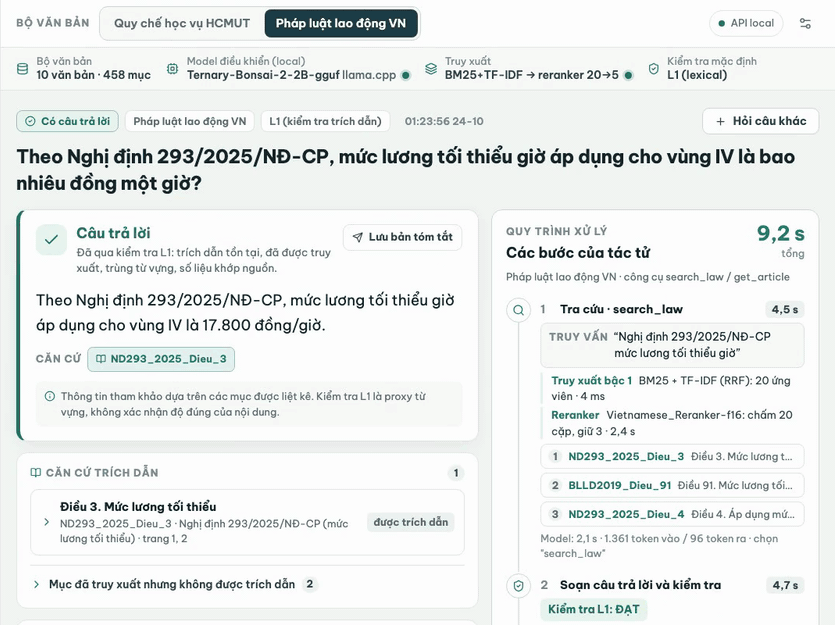
\includegraphics[width=\linewidth]{images/demo_answer.png}\\[2pt]{\small (b) Web interface, same question.}
\end{minipage}
\caption{(a) One completed trial from the evaluation (a labour-law question about the hourly minimum wage, seed 42). (b) The web interface answering the same question, showing the answer, citation verifier status, highlighted source section and step timeline.}\label{fig:trace}
\end{figure}



\section{Tools and Permissions}\label{sec:tools}
Table~\ref{tab:tools} lists every tool and model-facing interface with its implementation status and permission level. The controller's action schema contains no write action, leaving no direct write path from model output. All non-read-only interfaces are restricted or gated in Python rather than by prompt instructions alone. Although the main agent loop calls the Python tool registry directly, an accompanying Model Context Protocol (MCP) server exposes the same interfaces and is tested for tool discovery, retrieval, blocked unverified writes, and proposal-only summaries. The demo serves a single local user per process; multi-user isolation is not certified.
\begin{table}[!htbp]\tabstyle
% PROVENANCE: n/a descriptive tool inventory, no measured values
\begin{tabularx}{\textwidth}{@{}L{3.3cm}L{2.2cm}L{2.5cm}Y@{}}
\toprule Interface & State & Permission level & Enforced boundary\\\midrule
Corpus search and read tools & Implemented, used & Read-only & Return local corpus text only.\\
Reranker (inside search) & Implemented, used & Read-only model component & Scores candidates; a failure is an execution error, never a silent fallback.\\
Answer-memory write & Implemented, off in all runs & Reversible write & Local database write only after the verification gate.\\
Case-saving tool of the MCP server & Implemented, blocked & Reversible write & A model caller cannot self-attest verification; the call returns blocked.\\
Summary-sending tool & Proposal only & Irreversible write & The model-facing tool only creates a proposal; it cannot approve or execute.\\
Trusted-UI outbox & Implemented & Irreversible write (local queue) & Needs host approval and a token bound to the payload hash; a queue receipt is not a delivery.\\
External sender, code execution & Not implemented & Irreversible write, code execution & No e-mail or webhook transport and no code-running tool exists.\\
\bottomrule\end{tabularx}
\caption{Tool inventory with permission levels as classified in code.}\label{tab:tools}
\end{table}



\section{Memory and Knowledge Sources}\label{sec:memory}
\hdr{Short-term context.} Each run maintains a single message list: the domain system prompt, the user question (and any pasted document) wrapped as untrusted input, followed by alternating action and observation turns. Tool observations are compacted: a search returns the best-matching clauses of each record with a truncation flag, a repeated query or document read returns a brief notice, and step-budget notices prompt the controller to conclude with an answer or refusal before reaching the step limit. The controller uses an 8,192-token context window, and a case ledger records queries, retrieved IDs, repairs, token counts, and latencies.

\hdr{Long-term memory (implemented, disabled in all benchmark runs).} Verified answers can be stored in a local SQLite database after passing the verification gate. Reuse requires a matching index version and a question similarity of at least 0.85, and any retrieved answer is re-verified before return. Long-term memory is disabled across all benchmark runs and in the live demo so that trials remain independent and cached answers cannot ignore case-specific facts. Before any database write, regex filters screen out personal identifiers.

\hdr{Knowledge sources.} Both corpora were built from public PDFs by text extraction, Unicode NFC normalisation, and segmentation at article or section headings. Each record stores its source URL, SHA-256 file hash, and page numbers, with each article or section serving as the retrieval unit. The HCMUT corpus comprises 10 documents and 143 records (five documents are amendment-only, image-only base regulations are omitted, and decision numbers come from a web listing). The labour-law corpus comprises 10 documents and 458 records (Decree 145/2020 and unnumbered annexes are omitted, and texts reflect their promulgated versions without tracking later amendments). Neither corpus has been reviewed by an external legal or academic-affairs specialist.

\hdr{Retrieval and preliminary dense-vector probe toward D3.} At start-up, BM25 (over title and content) and word 1--3-gram TF-IDF indices are built in memory and fused by RRF; the top 20 candidates are rescored by a Vietnamese cross-encoder reranker (articles $>1{,}500$ chars are scored by their best overlapping window), and the first search always anchors on the user's raw question plus the model's query. To prepare for the D3 retrieval ablation, we integrated a persistent hybrid index combining \texttt{SQLite FTS5} with \texttt{EmbeddingGemma-2} (270M text backbone, \texttt{bfloat16} on MPS, $\approx 517$\,MB weights; \texttt{NumPy}/\texttt{FAISS}/\texttt{Qdrant} stores, $<6$\,MB on disk) into the codebase and demo UI. In a standalone probe on the two D2 corpora and an 818-query Vietnamese legal test set (\texttt{zalo\_legal\_hard1k}: 447 gold articles + 553 BM25 hard negatives from 61,425 Zalo AI legal articles), three findings emerged: (i)~\emph{pure dense embedding trails lexical search on statutes} (768-d vector-only reaches 52.9\% Recall@1 and 66.1\% MRR@10 vs.\ 62.5\%/75.4\% for \texttt{BM25+TF-IDF} and 68.8\%/80.2\% for \texttt{FTS5}), as statutory queries hinge on exact numeric/decree anchors whereas multilingual embeddings suffer from \emph{topic crowding} across adjacent clauses; (ii)~\emph{Matryoshka 128-d truncation hurts clause precision} ($-13.0$\,pp R@1 to 40.0\%, $-14.7$\,pp R@5 to 69.0\%) with no encoding speedup; and (iii)~\emph{weighted hybrid RRF ($0.75\,\text{FTS5} + 0.25\,\text{Vector}_{768\text{d}}$) outperforms both}, achieving \textbf{69.1\% Recall@1, 97.0\% Recall@5, 99.5\% Recall@20, and 80.9\% MRR@10} on \texttt{zalo\_legal\_hard1k} (vs.\ 67.0\% R@1 for unweighted 1:1 RRF) and 94.1--95.8\% MRR@10 on the D2 corpora.


\section{Evaluation Set and First Results}\label{sec:eval}
\hdr{Benchmarks.} Each self-built benchmark has 50 Vietnamese questions over its corpus (100 now; final target adds 50--100 unseen harder questions and $\ge$30 attack cases, Section~\ref{sec:plan}): 40 single-record, 5 two-record and 5 out-of-scope questions to refuse. Each comes with gold records, a reference answer and verbatim quotes, locked by hash before collection.

An AI model drafted the questions; two independent AI verifiers and an AI adjudicator cross-checked them; mechanical checks confirmed that every quote is verbatim. Then group member Võ Phạm Tuấn Dũng reviewed all 100 questions on 23 October and requested no change. They are AI-written questions over real documents, not real users' questions. A quality audit found no wrong gold answer and three limits:
\begin{itemize}
\item plain BM25 on the raw question already ranks a gold record first for 89\% (HCMUT regulations) and 78\% (labour law) of questions, so retrieval cannot separate the configurations;
\item about one third of the answerable questions can be answered without the corpus (LLM estimate);
\item 22 HCMUT questions pin a document by a decision number taken from a web listing.
\end{itemize}

\hdr{How success is decided.} \emph{Strict success} counts a trial only if the run completed, the behaviour was appropriate (answer when the corpus answers, refuse when it does not), the answer is judged correct and complete, and every factual claim is supported by the sources. Execution errors and failed judgments count as failures, so the rate is a lower bound over all planned trials. It is an LLM estimate, not a human label.

Three measures need no judge: behaviour match, over-refusal and unsafe answers. Recall@5 (are the gold documents among the agent's results?) and citation F1 (are the cited documents the gold ones?) are measured on document ids. They say nothing about answer correctness. Intervals are 95\% bootstrap intervals over questions, with the three seeds averaged per question. With 50 questions, differences below about 10 percentage points are not detectable. Definitions are in the repository.

\hdr{LLM judge and its check.} An LLM judge (DeepSeek V4 Flash, through an API gateway) rates each output blind to the configuration and verifier outcome (offline only; model revision not fixed~\citep{deepseek2026api}; LLM judges can be biased~\citep{zheng2023judge}). On a blind 60-item human audit (30 per benchmark, current 4B outputs), strict-success agreement is 96.7\% (29/30, $\kappa = 0.93$; weighted 98.8\%, $\kappa_w = 0.97$) on HCMUT and 90.0\% (27/30, $\kappa = 0.80$; weighted 97.5\%, $\kappa_w = 0.95$) on labour law; behaviour agreement is 100.0\% and 93.3\% ($\kappa=0.84$). All four disagreements are documented in the repository. Separating correctness from citation support follows~\citet{gao2023alce}.

\hdr{Design.} The full system (verifier and reranker) is compared with two simpler configurations: \emph{no verifier} (neither verifier nor reranker) and \emph{verifier} (verifier with repair, no reranker). Each runs three seeds on 50 questions per benchmark.

Two diagnostic baselines (one seed; they are not system variants) bracket the results: \emph{closed-book} (the question only, no tools or documents) and \emph{oracle} (the gold records given up front, answerable questions only). One controller thus has 900 system trials plus 190 baseline trials, 1{,}090 in all, every one recorded. The initial system and the current system with the 2B controller were run the same way. Accuracy was collected on a shared server GPU (one NVIDIA H100). Latency is measured separately on an Apple M4 laptop (16\,GiB), one query at a time.

\begin{figure}[!tbp]\centering
% PROVENANCE: comparison=evaluation/comparisons/v3-2B_vs_r2-2B_vs_r2-4B (comparison.json: table.<benchmark>.<variant>.arms.<arm>.strict_success and strict_success_ci95, 3 variants x 2 benchmarks x 3 arms)
\begin{tikzpicture}
\pgfplotsset{barax/.style={ybar,bar width=6.5pt,width=8.0cm,height=5.0cm,ymin=0,ymax=100,ytick={0,20,40,60,80,100},
  ymajorgrids,grid style={black!12},tick label style={font=\scriptsize},label style={font=\small},title style={font=\small\bfseries,yshift=-2pt},
  symbolic x coords={off,l1,lrr},xtick=data,xticklabels={no verifier,verifier,verifier + reranker},xticklabel style={align=center,text width=1.55cm,font=\scriptsize},enlarge x limits=0.22,
  error bars/y dir=both,error bars/y explicit,error bars/error bar style={black!80,line width=0.5pt}}}
\begin{axis}[barax,title={HCMUT regulations},ylabel={Strict success (\%)},legend to name=barlegend,legend columns=3,legend style={font=\scriptsize,draw=none,column sep=8pt}]
\addplot+[fill=cV,draw=black!55] table[x=v,y=y,y error plus=p,y error minus=m] {
v y p m
off 18.0 8.0 7.3
l1 12.0 6.0 5.3
lrr 14.0 7.3 6.0
};
\addplot+[fill=cR2,draw=black!55] table[x=v,y=y,y error plus=p,y error minus=m] {
v y p m
off 31.3 10.0 9.3
l1 24.0 9.3 8.7
lrr 28.7 8.7 8.7
};
\addplot+[fill=cR4,draw=black!55] table[x=v,y=y,y error plus=p,y error minus=m] {
v y p m
off 70.0 9.3 9.3
l1 64.0 10.7 11.3
lrr 60.7 10.0 10.7
};
\legend{{Initial system, 2B},{Current system, 2B},{Current system, 4B}}
\end{axis}
\begin{axis}[barax,title={Labour law},at={(9.0cm,0)},yticklabels={}]
\addplot+[fill=cV,draw=black!55] table[x=v,y=y,y error plus=p,y error minus=m] {
v y p m
off 14.7 8.0 7.3
l1 14.7 8.0 7.3
lrr 18.7 8.0 7.3
};
\addplot+[fill=cR2,draw=black!55] table[x=v,y=y,y error plus=p,y error minus=m] {
v y p m
off 31.3 9.3 9.3
l1 28.0 10.0 9.3
lrr 28.0 9.3 9.3
};
\addplot+[fill=cR4,draw=black!55] table[x=v,y=y,y error plus=p,y error minus=m] {
v y p m
off 62.0 10.0 10.0
l1 52.7 10.7 10.0
lrr 56.7 10.0 10.0
};
\end{axis}
\end{tikzpicture}\\[1pt]
\pgfplotslegendfromname{barlegend}
\caption{Strict success (LLM-judge lower bound; bars: mean over three seeds; whiskers: 95\% interval over the 50 questions) for the initial system with the 2B controller and the current system with the 2B and 4B controllers. The right-most group, verifier + reranker, is the full system; with the 4B controller it is the current system we propose. The current system was revised after we analysed the initial system's failures on these same questions.}\label{fig:bars}
\end{figure}


\hdr{What the numbers say.}\par\noindent\textbf{(1) Controller scale and loop design both matter, and model scale matters most} (Figure~\ref{fig:bars}). For the full system (\emph{verifier + reranker}), strict success is 60.7\% [50--71] on HCMUT regulations and 56.7\% [47--67] on labour law with the 4B controller, compared with 28.7\% and 28.0\% with the 2B controller (and 14.0\% and 18.7\% on the early 2B prototype).

Upgrading the controller from 2B to 4B on the same D2 pipeline adds $+32.0$ percentage points [21.3, 42.0] on HCMUT and $+28.7$ [18.0, 39.3] on labour law, while the query-anchoring and verifier refinements at 2B added $+14.7$ [6.0, 23.3] and $+9.3$ [0.7, 18.0]. All twelve paired bootstrap differences across the three configurations exclude zero (full tables in the appendix).

\par\noindent\textbf{(2) The verifier and the reranker did not raise strict success.} In Table~\ref{tab:main}, the configuration without verifier is highest (70.0\% and 62.0\%). Adding the verifier changes strict success by $-6.0$ [$-16.0$, $+4.0$] and $-9.3$ [$-18.7$, $0.0$] points. Adding the reranker on top of the verifier changes it by $-3.3$ [$-13.3$, $+6.7$] and $+4.0$ [$-6.0$, $+14.0$].

Table~\ref{tab:diag} shows why: both make the system refuse more, because an answer the verifier rejects twice ends as a refusal (10 to 18 of 150 trials per configuration, always on questions where an answer was expected). Unsafe answers on the 15 out-of-scope trials per row do not fall consistently, from a very small base. Recall@5 is already 0.98--0.99 without the reranker. The full system keeps both components for the guarantee of a checkable citation. The final report tests on a harder, unseen set of questions whether the cost in refusals is justified.

\begin{table}[!htbp]\tabstyle
% PROVENANCE: run=d2-gpu-r2-4b-hcmut-v1,d2-gpu-r2-4b-labour-v1 (label required by the checker, invisible: post-hoc revision evaluated on the same tasks)
\begin{tabular}{@{}lcccc@{}}
\toprule & \multicolumn{2}{c}{HCMUT regulations} & \multicolumn{2}{c}{Labour law}\\\cmidrule(lr){2-3}\cmidrule(lr){4-5}
Current system, 4B controller & All 50 questions & 45 answerable & All 50 questions & 45 answerable\\\midrule
Closed-book (no documents) & 2.0 [0--6] & 0.0 [0--0] & 24.0 [12--36] & 24.4 [13--38]\\
No verifier, no reranker & 70.0 [61--79] & 69.6 [60--79] & 62.0 [52--72] & 60.7 [50--71]\\
Verifier (with repair) & 64.0 [53--75] & 61.5 [50--73] & 52.7 [43--63] & 51.1 [40--62]\\
\textbf{Verifier + reranker (full system)} & \textbf{60.7 [50--71]} & 59.3 [49--70] & \textbf{56.7 [47--67]} & 54.1 [43--64]\\
Oracle (gold records given up front) & -- & 82.2 [71--93] & -- & 75.6 [62--87]\\
\bottomrule\end{tabular}
\caption{Strict success (\%, LLM-judge lower bound, 95\% bootstrap interval over questions) of the D2 system with the 4B controller. Configurations: three seeds; closed-book and oracle: one seed. The oracle runs only on the 45 answerable questions, so the right-hand columns of each benchmark compare every row on the same 45 answerable questions.}\label{tab:main}
\end{table}

\begin{table}[!htbp]\tabstyle
% PROVENANCE: run=d2-gpu-r2-4b-hcmut-v1,d2-gpu-r2-4b-labour-v1 (label required by the checker, invisible: post-hoc revision evaluated on the same tasks)
\begin{tabular}{@{}llccccccc@{}}
\toprule Benchmark & Configuration & \makecell{Unverified\\cit.\ leak (\%)} & \makecell{Audited\\strict (\%)} & \makecell{Behaviour\\match (\%)} & \makecell{Over-\\refusal (\%)} & \makecell{Faithful-\\ness (\%)} & \makecell{Citation\\F1} & Recall@5\\\midrule
\multirow{3}{*}{HCMUT regulations} & No verifier & 25.6 & 55.3 & 88.0 & 9.8 & 89.8 & 0.820 & 0.989\\
 & Verifier & \textbf{0.0} & \textbf{64.0} & 82.7 & 17.4 & 90.3 & 0.704 & 0.989\\
 & Verifier + reranker & \textbf{0.0} & \textbf{60.7} & 80.0 & 18.9 & 89.3 & 0.714 & 0.978\\\midrule
\multirow{3}{*}{Labour law} & No verifier & 28.0 & 51.3 & 94.0 & 4.4 & 87.3 & 0.841 & 0.989\\
 & Verifier & \textbf{0.0} & 52.7 & 81.3 & 16.8 & 86.3 & 0.728 & 0.989\\
 & Verifier + reranker & \textbf{0.0} & \textbf{56.7} & 79.3 & 19.1 & 85.6 & 0.691 & 0.993\\
\bottomrule\end{tabular}
\caption{Ablation of the rule-based citation verifier and the reranker (4B controller, 3 seeds $\times$ 50 questions per row). \emph{Unverified cit.\ leak}: share of emitted answers whose quotes, section IDs or numbers fail deterministic source verification against the full PDF corpus (31/121 HCMUT and 37/132 labour answers in \emph{No verifier} vs 0/109 and 0/108 with the verifier). \emph{Audited strict}: trials that pass both the LLM judge and deterministic L1 citation verification. Behaviour match, Over-refusal, Citation F1 and Recall@5 need no judge.}\label{tab:diag}
\end{table}


\par\noindent\textbf{(3) Baselines.} Without documents the 4B model scores 2.0\% [0--6] on HCMUT regulations and 24.0\% [12--36] on labour law, so part of the labour-law score can come from the model's own knowledge. With the gold records in front of it, the oracle reaches 82.2\% [71--93] and 75.6\% [62--87] on the answerable questions. Even with perfect evidence the 4B controller misses strict success on about one question in five, against 69.6\% and 60.7\% for the agent without verifier on the same questions. 17 of 1,090 trials ended as execution errors (wall-time limit); they count as failures.

\hdr{Error analysis and scope limits.} Three failure modes account for the remaining errors in the 4B full system: (i) \emph{repair-budget refusals} (13/150 HCMUT and 18/150 labour trials refused after two L1 quote/number rejections on answerable questions), (ii) \emph{multi-clause synthesis omissions} (oracle gap of about 18--24\% even when gold articles are given up front), and (iii) \emph{wall-time budget timeouts} (17 of 1,090 trials). Because the engineering refinements in Section~\ref{sec:changes} were informed by failure traces on this 100-question set and lexical retrieval is near ceiling, we will evaluate generalization on a new unseen benchmark of harder multi-hop and paraphrased questions in Week 45.

\hdr{Cost and latency.} The controller and reranker run locally, so there is no per-call API cost. For the full system the controller reads on average 12,070 (HCMUT regulations) and 11,477 (labour law) tokens and writes 763 and 865 tokens per trial, over 3.4 and 3.7 model calls. The judge cost, as reported by the gateway and not an invoice, was USD 1.06 and USD 1.10 for the two 545-trial runs. Collecting a run took 34 and 33 minutes of wall time on the shared H100 (GPU-active hours were not measured). On the laptop (Apple M4, one question at a time, 50 questions per benchmark), the full system answers in a median of 33.0\,s (HCMUT regulations) and 29.8\,s (labour law) per question with the 4B controller (95th percentile 86\,s and 72\,s), and in 13.3\,s and 14.6\,s with the 2B controller (95th percentile 30\,s and 28\,s); the 4B model generates about 43 tokens/s, the 2B about 92.

\hdr{Reproducibility.} Repository: \url{https://github.com/tuandung222/LuatCheck-D2}; reported commit \texttt{138128e804bf}. All numbers and tables are regenerated from recorded runs by one command (\texttt{make report-check}); instructions are in the repository.


\section{Threat Model}\label{sec:threat}
\hdr{Assets.} (A1) Faithfulness: answers and citations that users rely on must trace to source sections~\citep{magesh2025hallucination}. (A2) User data: questions, pasted documents, memory and the audit log. (A3) Integrity of corpora, domain profiles, prompts, model weights and the frozen benchmark. (A4) The tool boundary: no unreviewed write or egress. (A5) Availability of a bounded local machine.

\hdr{Attacker.} The attacker can submit arbitrary questions and pasted documents through the interface or API (instruction override, delimiter spoofing, prompt or memory exfiltration, requests to evade a regulation), including text copied from a hostile third party. The attacker cannot change code, corpora, configuration, weights, the ledger or the approval state of the trusted UI, and cannot reach loopback servers or other users' sessions. Non-goals: a compromised host or supply chain, poisoned official sources, multi-tenant isolation, and the correctness of the regulations themselves.

\begin{table}[!htbp]\tabstyle
% PROVENANCE: n/a threat model table, no measured values
\begin{tabularx}{\textwidth}{@{}L{3.0cm}L{6.3cm}Y@{}}
\toprule Entry point (asset) & Mitigation & Residual risk\\\midrule
Question, pasted document (A1, A4) & Regex guardrails (shared and per-domain patterns) before any model call, Unicode and delimiter sanitising, untrusted-text tags, fixed action space without a write action & Paraphrases bypass patterns; Vietnamese and English only; false positives; no learned classifier; not attack-tested yet.\\
Retrieved text (A1) & Observations are tagged as tool results; the citation verifier checks ids, provenance and quotes & Tagged, not filtered: an instruction inside a source document would reach the model.\\
Ingested documents (A3) & Offline, manual ingestion; source URL, hash and pages per record; benchmark locks hash the corpora & No signature check; trust in the official site.\\
Memory (A1, A2) & Off in all runs and in the demo; index version, similarity, re-verification, personal-data patterns & Poisoning by an earlier user; incomplete personal-data filter.\\
Weights, configuration, binaries (A3) & Recorded hashes and commit, identity checks before each run, loopback-only endpoints & Third-party weights and the llama.cpp fork are not audited.\\
Judge gateway (A2) & Offline only; benchmark data only; key kept in the environment; blind packets; output validation; human audit & Candidate text could steer the judge (untested); model version not fixed.\\
Web interface, API, outbox, long inputs (A4, A5) & Loopback bind, session cookie and CSRF token, size limits; proposal-only tools with host approval; step, tool, repair, time limits & Single-user assumption; limits turn overload into errors, not into defences.\\
Web pages & Not applicable: there is no browsing tool. & --\\
\bottomrule\end{tabularx}
\caption{Threat model by entry point. Mitigations are implementation boundaries, not measured attack effectiveness. The full-system injection tests~\citep{greshake2023indirect,debenedetti2024agentdojo} belong to the final report (planned for week 47; no attack numbers in this report).}\label{tab:threat}
\end{table}



\section{Weekly Plan to the First Final Presentation}\label{sec:plan}
Table~\ref{tab:plan} runs to the first final presentation in week 49. The final phase focuses on harder unseen multi-hop questions, real-user feedback from the HR walkthrough, and entry-point prompt-injection testing.
\begin{table}[!htbp]\tabstyle
% PROVENANCE: n/a plan table, dates only
\begin{tabularx}{\textwidth}{@{}L{3.3cm}L{2.2cm}Y@{}}
\toprule Week (dates) & Owner & Deliverable and acceptance\\\midrule
24--25 Oct (Done) & Dũng, all & Blind human audit of the 60-item judge sample (30 per benchmark); agreement (96.7\% and 90.0\%) and $\kappa$ ($0.93$ and $0.80$) added to Section~\ref{sec:eval}.\\
Sun 25 Oct, Wed 28 Oct & Quyền (leader), all & Submit report and slides; presentation with live demo and backup video.\\
Week 45 (2--8 Nov) & Quyền, Phong & HR walkthrough with findings. Design and freeze a new benchmark of unseen, harder questions (scenario, multi-hop, conditional and temporal, paraphrased), reviewed by members.\\
Week 46 (9--15 Nov) & Dũng, Quyền & Run the current system and its ablations on the new benchmark; add the dense-retrieval ablation; failure analysis.\\
Week 47 (16--22 Nov) & Phong, Dũng & Entry-point attack tests; permission and fault checks.\\
Week 48 (23--29 Nov) & All & Reproduction from the recorded runs, demo hardening, final report.\\
Week 49 (30 Nov--2 Dec) & All & Tagged release and Round 1 presentation on 2 December.\\
\bottomrule\end{tabularx}
\caption{Weekly plan to the first final presentation, with assigned owners.}\label{tab:plan}
\end{table}

\hdr{Riskiest assumption and fallback.} The riskiest assumption is that a small 2--4B local controller maintains high strict accuracy on harder, unanchored questions (paraphrased scenarios that do not name the decision or decree number) without exceeding the 2-repair budget. If strict success drops sharply on the new benchmark or dense retrieval and NLI verification do not improve over the current pipeline, we keep the bounded loop, the L1 citation verifier, the two corpora and the evaluation harness as the core deliverable, report the measured numbers transparently, and drop the optional NLI check and extra domains.

\hdr{Self-assessment: on track.} The end-to-end system, both corpora, the 100-question evaluation suite, the 60-item human audit of the judge, and the one-command reproduction pipeline are complete, reaching 57--61\% strict success with the full 4B system. The remaining tasks for the final report are the unseen harder benchmark (W45--W46) and red-team attack evaluation (W47).


\section{Member Contributions and AI-Use Statement}\label{sec:contrib}
\begin{table}[H]\tabstyle
% PROVENANCE: n/a contribution table, no measured values
\footnotesize\renewcommand{\arraystretch}{1.08}
\begin{tabularx}{\textwidth}{@{}L{2.8cm}cL{3.2cm}Y@{}}
\toprule Member & Contrib. & Role in the proposal & Completed work and repository evidence\\\midrule
Lê Trí Quyền (Group Leader) & 33\% & Retrieval and serving: ingestion, BM25 + dense index, RRF, reranking, local deployment & Corpus ingestion and normalisation (\texttt{src/ingestion/}), BM25 + TF-IDF and vector indexing with RRF fusion (\texttt{src/indexing/}), cross-encoder reranker integration (\texttt{src/retrieval/}), \texttt{llama.cpp}/Prism local serving and cross-platform Docker deployment (commits \texttt{555919a}, \texttt{8fed7c5}, \texttt{15fd823}, \texttt{ad0881b}, \texttt{bdb5d69}, \texttt{415efda}).\\
Võ Phạm Tuấn Dũng (Technical Lead) & 33\% & Agent, architecture and evaluation: system design, model selection, control loop, verifier and evaluation & Idea proposal and verification, system architecture and local model selection, codebase organisation and refactoring; bounded ReAct control loop and config-driven pipeline (\texttt{src/agent/}, \texttt{src/pipeline/}), L1 citation verifier and bounded repair (\texttt{src/verifier/}), 100-task benchmarks (\texttt{evaluation/benchmarks/}), evaluation harness, GPU/Mac runs, 60-item judge audit, statistical analysis and D2 report/slides (all remaining commits in the repository).\\
Nguyễn Hoàng Phong & 33\% & System and security: tool layer, UI, audit log, persistent store, fault and injection harness & Tool registry and code-enforced permissions (\texttt{src/tools/}), regex guardrails and PII filtering (\texttt{src/security/}), Web and Streamlit interfaces with trusted outbox (\texttt{frontend/}, \texttt{src/api/}, \texttt{src/ui/}), SQLite store and audit ledger (\texttt{src/memory/}), and fault/security test suites (commits \texttt{6dc1dbc}, \texttt{78bb069}, \texttt{2c1f3d0}, \texttt{d117349}, \texttt{7ce7e45}, \texttt{1272dc7}, \texttt{e0b4a05}, \texttt{edc9bfa}).\\
\bottomrule\end{tabularx}
\caption{Member contributions (equal 33\% split) matched to proposal responsibilities, repository modules and commit history.}\label{tab:contrib}
\end{table}


\hdr{AI-use statement.} The group used a range of AI models from Anthropic (Claude), Google (Gemini, Gemma) and OpenAI (Codex) for discussion and execution support. The problem framing, system scope, design decisions, task assignment to coding agents, supervision and code review were done by the group; every change was reviewed and approved by a group member before it was committed. AI coding agents implemented code from specifications written or approved by the group. AI models were also used, under the group's direction, to draft and cross-check benchmark questions (all questions were then reviewed by a group member), to act as the evaluation judge (an LLM estimate, checked against the group's human audit), and to draft analyses and report text that the group edited.

\hdr{Verified by the group.} Võ Phạm Tuấn Dũng reviewed all 100 benchmark questions against the source PDFs (23 October), audited the 60-item blind judge sample (25 October: 96.7\% agreement, $\kappa=0.93$ on HCMUT; 90.0\%, $\kappa=0.80$ on labour law), verified the architecture and code across all commits, and checked the Mac demo runs. Lê Trí Quyền verified corpus extraction, BM25/TF-IDF indexing and local \texttt{llama.cpp}/reranker serving. Nguyễn Hoàng Phong verified tool permission boundaries, guardrails and Web UI states. Automated tests use real components and no mocks (425 passed, 2 skipped, 1 failed needing an unstarted Ollama backend).


\begingroup\footnotesize\setlength{\bibsep}{1pt plus 0.5pt}
\bibliography{refs}\endgroup

\end{document}
